\begin{sectionblock}{Multiple Textbooks}

  Tagging an open-source linear algebra textbook with the
  CuratedCourses taxonomy enables the margin of the textbook to be populated with relevant open
  resources.\\[1ex]

  And not only can resources be aligned to textbooks, but the textbooks can also be aligned with each other.

  \begin{figure}
    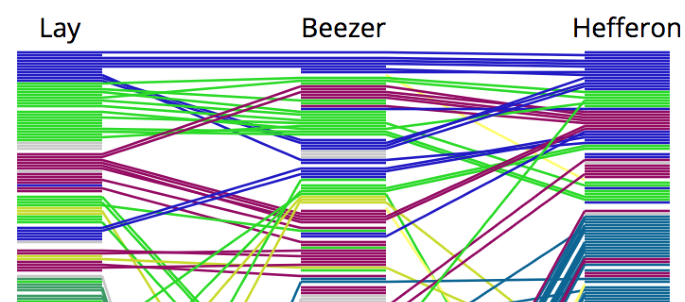
\includegraphics[width=0.9\textwidth]{alignment.pdf}
  \end{figure}


\end{sectionblock}



\begin{sectionblock}{Workshop and Minicourse}
  As part of the project, the team runs workshops to train
  faculty in the development of and the use of open content, including
  a minicourse at the Joint Math Meetings in January 2018 and a
   workshop in August 2018.


\end{sectionblock}


